\documentclass{standalone}
%outline around text
\usepackage[outline]{contour}
\contourlength{1.3pt}

%tikz
\usepackage{tikz}
\usetikzlibrary{knots, cd, calc}

\begin{document}
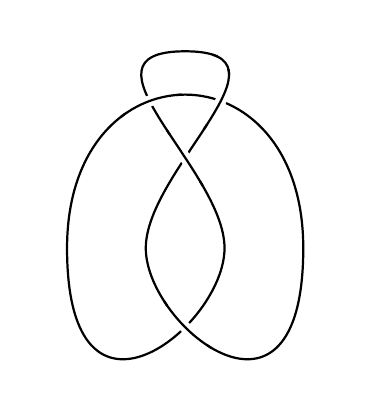
\begin{tikzpicture}
\clip (-2, -2.5) rectangle (2, 1.8);
\begin{knot}[consider self intersections = true, ignore endpoint intersections=false, clip width = 5, flip crossing = 2]
\strand[thick] (0, 1.5) .. controls +(1.5, 0) and +(0, 1) .. (-0.5, -1) .. controls +(0, -1) and +(0, -2.6) .. (1.5, -1) .. controls +(0, 2.6) and +(0, 2.6) .. (-1.5, -1) .. controls +(0, -2.6) and +(0, -1) .. (0.5, -1) .. controls +(0, 1) and +(-1.5, 0) .. (0, 1.5);
\end{knot}
\end{tikzpicture}
\end{document}



